\chapter{Pression, énergie libre et fluctuations de l’énergie}

\lectureoverview{Nous déduisons la pression de la fonction de partition sans recourir à une représentation cinétique des molécules heurtant une paroi. Un lemme géométrique transforme une dérivée adiabatique en dérivées à température fixe, l’énergie libre de Helmholtz fournit le lien avec \(\log Z\), et la loi des gaz parfaits en découle comme première application. Nous utilisons ensuite la même fonction de partition pour déduire les fluctuations de l’énergie à l’équilibre et leur relation avec la capacité thermique.}

\section{Laissons les mathématiques éprouver notre intuition}

La thermodynamique a une réputation singulière. Son calcul différentiel est élémentaire, mais le choix de la grandeur à dériver et de celle à maintenir fixe peut être remarquablement subtil. Notre problème est volontairement circonscrit : calculer la pression d’un gaz parfait. La démarche qui mène à la réponse se veut toutefois assez générale pour s’appliquer à des systèmes où l’image familière des molécules n’est plus fiable.

L’explication cinétique est facile à donner. Les molécules frappent une paroi et inversent la composante normale de leur quantité de mouvement. La quantité de mouvement transférée par unité de temps donne la force, et la force par unité de surface donne la pression. Nous savons déjà que l’énergie cinétique moyenne par molécule en trois dimensions vaut \begin{equation}
 \left\langle \frac{p^2}{2m}\right\rangle=\frac{3}{2}T
 \qquad (k_B=1).
 \label{eq:sm5-mean-kinetic-energy}
\end{equation}Avec une distribution isotrope des vitesses, on peut estimer la fréquence des collisions, le transfert de quantité de mouvement à chaque collision et la pression qui en résulte.

Mais la paroi elle-même semble rompre l’isotropie. Pourquoi les molécules très proches de la frontière auraient-elles la même distribution de vitesses et de directions que celles situées profondément à l’intérieur ? À l’équilibre, c’est bien le cas, avec la précision pertinente ici, mais cette conclusion devrait découler de la mécanique statistique plutôt que d’être introduite subrepticement dans le calcul au nom de l’intuition. Les collisions entre molécules rendent l’argument cinétique encore moins transparent. Le gaz sans interactions est facile à traiter précisément parce qu’il s’agit d’un système exceptionnellement simple.

En physique, il arrive que la démarche la plus sûre consiste à mettre provisoirement de côté les images intuitives et à suivre les mathématiques. On identifie la grandeur à déterminer, on manipule les relations générales et on attend qu’apparaisse une formule reconnaissable. L’intuition revient à la fin, mais les mathématiques éprouvent alors l’intuition, et non l’inverse. Le plaisir de la thermodynamique tient aux relations surprenantes qui émergent de cette démarche.

La relation recherchée est une équation d’état, \begin{equation}
 P=P(T,V,N),
 \label{eq:sm5-equation-of-state-target}
\end{equation} où \(N\) désigne la quantité de matière, \(T\) la température et \(V\) le volume. Une dérivation satisfaisante devrait rester valable lorsque les particules interagissent, ou lorsque la matière est un liquide, un plasma ou un solide. Seul le calcul final de la fonction de partition sera propre au gaz parfait.

\section{Entropie et énergie libre de Helmholtz}

Commençons par rappeler les formules canoniques dont nous aurons besoin plus tard. Pour des microétats indexés par \(i\), \begin{equation}
 \begin{aligned}
 S&=-\sum_i p_i\log p_i,\\
 p_i&=\frac{e^{-\beta E_i}}{Z},\\
 Z&=\sum_i e^{-\beta E_i}.
 \end{aligned}
 \label{eq:sm5-canonical-definitions}
\end{equation} Le logarithme de la probabilité est \begin{equation}
 \log p_i=-\beta E_i-\log Z.
 \label{eq:sm5-log-probability}
\end{equation} En substituant dans l’expression de l’entropie, on obtient \begin{align}
 S
 &=-\sum_i p_i\log p_i \notag\\
 &=\beta\sum_i p_iE_i+\log Z\sum_i p_i \notag\\
 &=\beta E+\log Z.
 \label{eq:sm5-entropy-log-z}
\end{align} Ici, \(E=\sum_i p_iE_i\) désigne l’énergie moyenne.

\begin{classroomqa}\audiencequestion{Pourquoi le second terme ne donne-t-il que \(\log Z\), et non le nombre d’états multiplié par \(\log Z\) ?}\lecturerresponse{Le coefficient que l’on somme est \(p_i\), et non \(1\). La normalisation donne \(\sum_i p_i=1\). De façon équivalente, le numérateur \(\sum_i e^{-\beta E_i}=Z\) se simplifie avec le \(Z\) du dénominateur. Le nombre d’états n’intervient jamais dans cette étape.\lecturetimestamp{00:14:25--00:14:55}}\end{classroomqa}

Dans les unités d’énergie utilisées pendant la majeure partie du cours, \(\beta=1/T\). En multipliant \eqref{eq:sm5-entropy-log-z} par \(T\) et en réarrangeant, on obtient \begin{equation}
 E-TS=-T\log Z.
 \label{eq:sm5-helmholtz-identity}
\end{equation} La combinaison qui figure à gauche apparaît si souvent qu’elle mérite un nom : \begin{equation}
 A\equiv E-TS,
 \qquad
 A=-T\log Z.
 \label{eq:sm5-helmholtz-definition}
\end{equation} C’est l’énergie libre de Helmholtz. Pour l’instant, son nom importe moins que l’identité elle-même ; nous en aurons besoin pour exprimer la pression comme une dérivée de la fonction de partition.

\begin{figure}[t]\centering
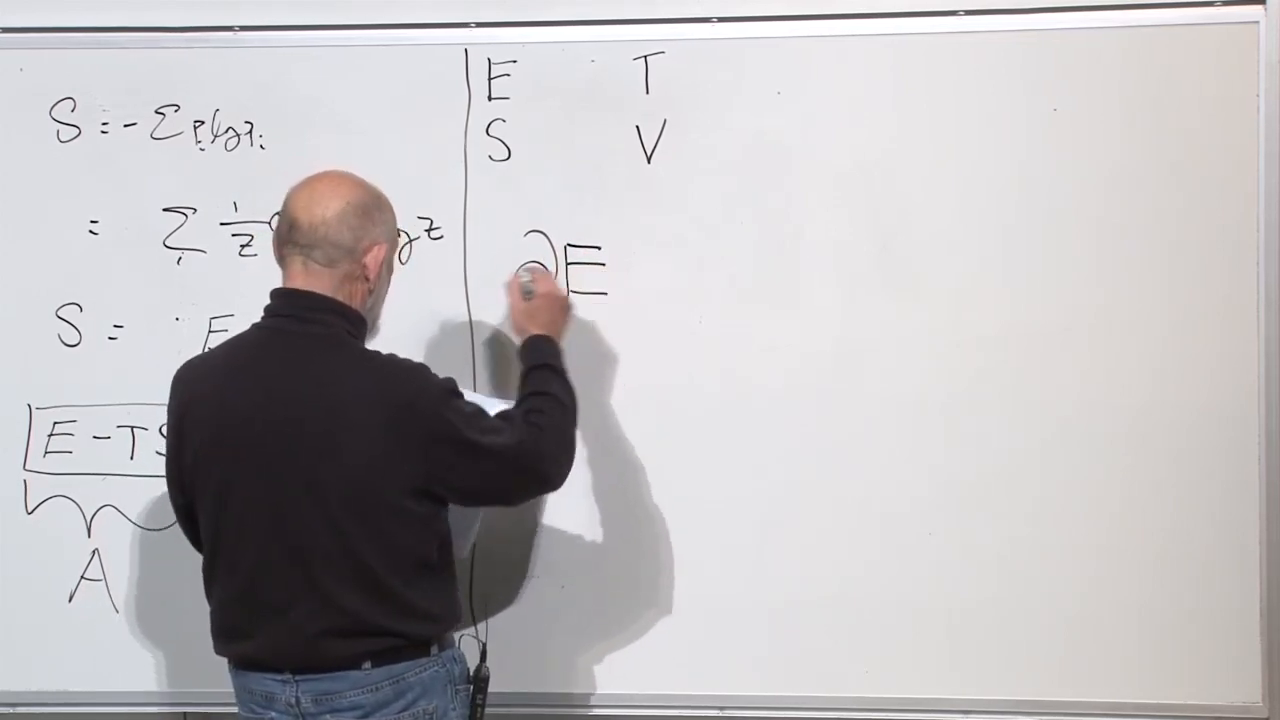
\includegraphics[width=0.90\textwidth]{lecture_05_figure_03.png}\caption{La relation canonique de l’entropie réécrite sous la forme \(A=E-TS=-T\log Z\).}\lectureframe{00:16:50}\end{figure}

\section{Paramètres de contrôle et réponses du système}

Un paramètre de contrôle est une grandeur macroscopique qu’un expérimentateur peut modifier de l’extérieur. Déplacer un piston change le volume sans manipuler les molécules une à une. Les champs électriques et magnétiques appliqués en sont d’autres exemples. Dans un ensemble plus général, le nombre de particules peut lui aussi varier.

Les variables thermodynamiques vont naturellement par paires conjuguées. Dans le problème présent, le volume est le paramètre de contrôle et la pression est la réponse du système. Nous faisons varier \(V\) ; la pression indique la résistance énergétique du système à cette variation. La dérivée de l’énergie précisera plus tard cette association.

\begin{classroomqa}\audiencequestion{Peut-on considérer la pression elle-même comme le paramètre de contrôle ?}\lecturerresponse{On peut concevoir une expérience où la pression extérieure est maintenue fixe, mais dans le montage utilisé ici, la position du piston fixe le volume et la pression intérieure est la réponse du système. La pression et le volume sont des variables conjuguées ; celle que l’on contrôle dépend de l’ensemble et du dispositif expérimental.\lecturetimestamp{00:19:22--00:20:01}}\end{classroomqa}

\begin{classroomqa}\audiencequestion{Suppose-t-on que toutes les molécules sont identiques, ou le raisonnement se limite-t-il à un gaz ?}\lecturerresponse{L’argument thermodynamique n’exige aucune restriction de ce genre. Le cylindre peut contenir plusieurs espèces, un liquide ou même un solide que l’on comprime. La fonction de partition du gaz parfait ne constituera qu’une application particulière, une fois établie la formule générale de la pression.\lecturetimestamp{00:20:02--00:20:39}}\end{classroomqa}

\begin{classroomqa}\audiencequestion{Peut-on aussi modifier la quantité de matière par une autre opération extérieure ?}\lecturerresponse{Oui. Le nombre de particules est un autre paramètre de contrôle possible. Le traiter comme une variable conduit à sa propre variable conjuguée : le potentiel chimique. Pour le calcul de ce soir, \(N\) reste fixe.\lecturetimestamp{00:20:39--00:20:57}}\end{classroomqa}

\begin{classroomqa}\audiencequestion{De l’eau liquide et de la vapeur peuvent-elles coexister à l’équilibre ?}\lecturerresponse{Oui, à la température et à la pression de coexistence. La gravité peut placer le liquide sous la vapeur, mais les deux phases peuvent malgré tout être à la même température et rester en équilibre thermique. Le même cadre général de la mécanique statistique s’applique.\lecturetimestamp{00:20:59--00:21:36}}\end{classroomqa}

Pour le raisonnement qui suit, considérons l’énergie et l’entropie comme des fonctions dépendantes de deux variables que l’on peut régler indépendamment : \begin{equation}
 E=E(T,V),
 \qquad
 S=S(T,V).
 \label{eq:sm5-dependent-functions}
\end{equation} La température et le volume servent de coordonnées dans l’espace des états thermodynamiques. L’énergie et l’entropie attribuent une valeur à chaque point d’équilibre de cet espace.

\section{La dérivée à entropie constante}

La dérivée dont nous aurons finalement besoin est inhabituelle : \[
 \left(\frac{\partial E}{\partial V}\right)_S.
\] Bien que \(T\) et \(V\) soient les coordonnées indépendantes, cette dérivée consiste à faire varier \(V\) tout en imposant à la fonction dépendante \(S(T,V)\) de rester constante. C’est une dérivée le long d’une courbe dans le plan \((T,V)\), et non le long d’un axe de coordonnées.

\begin{classroomqa}\audiencequestion{Comment \(T\) et \(V\) peuvent-ils être indépendants si l’on utilise ensuite la dérivée \(dT/dV\) ?}\lecturerresponse{Ils sont indépendants dans l’ensemble de l’espace des états. Dès que l’on impose la contrainte \(S(T,V)=\mathrm{constant}\), les états accessibles se trouvent sur une courbe unidimensionnelle. Le long de cette courbe, \(T\) devient une fonction de \(V\), et sa pente \(dT/dV\) est bien définie.\lecturetimestamp{01:01:18--01:02:09}}\end{classroomqa}

\begin{lemma}Si \(E(T,V)\) et \(S(T,V)\) sont différentiables, alors, partout où \((\partial S/\partial T)_V\neq0\), \begin{equation}
 \left(\frac{\partial E}{\partial V}\right)_S
 =
 \left(\frac{\partial E}{\partial V}\right)_T
 -
 \left(\frac{\partial E}{\partial S}\right)_V
 \left(\frac{\partial S}{\partial V}\right)_T.
 \label{eq:sm5-calculus-lemma}
\end{equation}\end{lemma}

\begin{proof}Pour un déplacement infinitésimal arbitraire, \begin{equation}
 dE=
 \left(\frac{\partial E}{\partial V}\right)_T dV
 +
 \left(\frac{\partial E}{\partial T}\right)_V dT.
 \label{eq:sm5-total-differential-e}
\end{equation} À \(V\) fixé, la règle de la chaîne permet d’introduire \(S\) comme variable intermédiaire : \begin{equation}
 \left(\frac{\partial E}{\partial T}\right)_V
 =
 \left(\frac{\partial E}{\partial S}\right)_V
 \left(\frac{\partial S}{\partial T}\right)_V.
 \label{eq:sm5-chain-rule-e-s-t}
\end{equation}

Limitons maintenant le déplacement à une courbe sur laquelle \(S\) est constante. Le long de cette courbe, \begin{equation}
 0=dS=
 \left(\frac{\partial S}{\partial V}\right)_T dV
 +
 \left(\frac{\partial S}{\partial T}\right)_V dT.
 \label{eq:sm5-constant-entropy-differential}
\end{equation} En isolant la pente de la courbe, on obtient \begin{equation}
 \left(\frac{dT}{dV}\right)_S
 =
 -
 \frac{\left(\frac{\partial S}{\partial V}\right)_T}
 {\left(\frac{\partial S}{\partial T}\right)_V}.
 \label{eq:sm5-entropy-contour-slope}
\end{equation} Divisons \eqref{eq:sm5-total-differential-e} par \(dV\), utilisons \eqref{eq:sm5-chain-rule-e-s-t} et introduisons \eqref{eq:sm5-entropy-contour-slope} : \begin{align}
 \left(\frac{\partial E}{\partial V}\right)_S
 &=
 \left(\frac{\partial E}{\partial V}\right)_T
 +
 \left(\frac{\partial E}{\partial S}\right)_V
 \left(\frac{\partial S}{\partial T}\right)_V
 \left(\frac{dT}{dV}\right)_S \notag\\
 &=
 \left(\frac{\partial E}{\partial V}\right)_T
 -
 \left(\frac{\partial E}{\partial S}\right)_V
 \left(\frac{\partial S}{\partial V}\right)_T.
\end{align} Le facteur \((\partial S/\partial T)_V\) s’est simplifié, ce qui démontre le résultat.\end{proof}

\begin{figure}[t]\centering
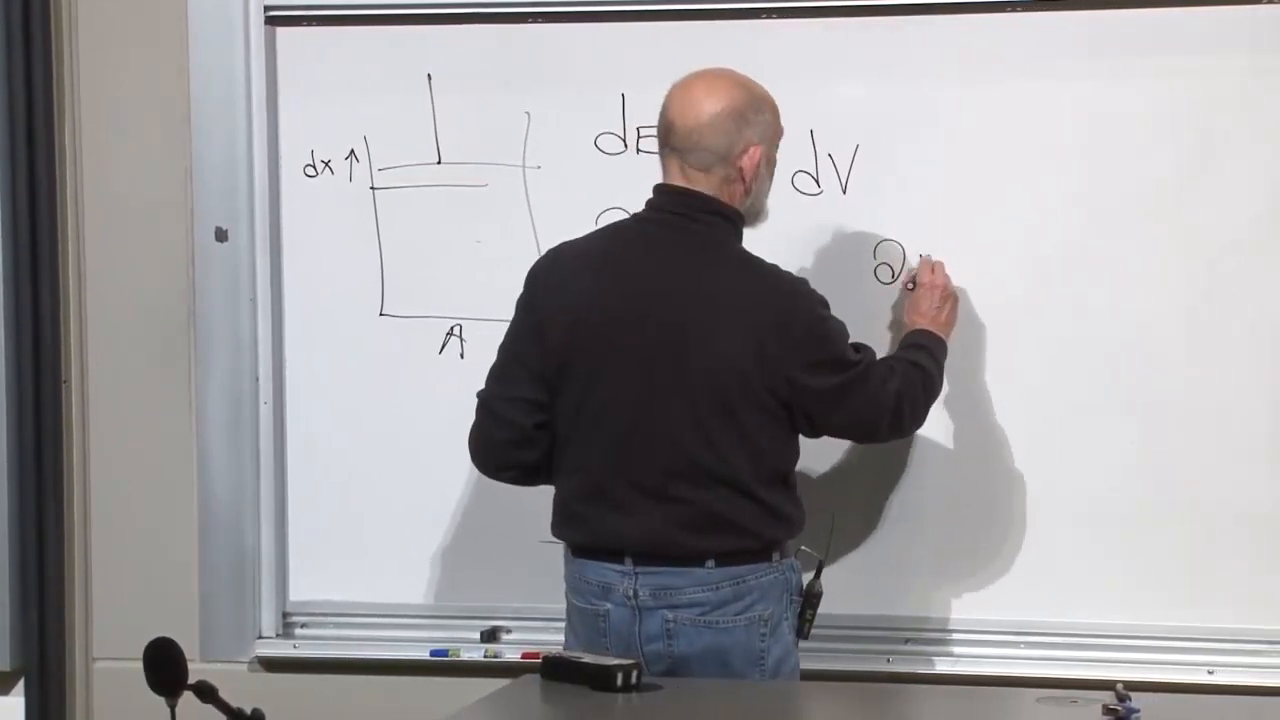
\includegraphics[width=0.90\textwidth]{lecture_05_figure_04.png}\caption{Calcul le long d’une courbe à entropie constante, au stade de la simplification qui achève le lemme sur la dérivée.}\lectureframe{00:36:10}\end{figure}

La représentation géométrique n’est pas décorative. Elle explique pourquoi une dérivée à \(S\) fixé, qui semble étrange, peut se calculer à l’aide des dérivées partielles ordinaires par rapport aux coordonnées indépendantes \(T\) et \(V\). Écrire \(\delta E/\delta V\) pendant la construction rappelle utilement que les symboles représentent des rapports de petites variations le long d’un chemin spécifié.

\begin{classroomqa}\audiencequestion{Le développement de \(dE\) correspond-il simplement à la définition ordinaire des dérivées partielles ?}\lecturerresponse{Oui. Le différentiel total ne présente rien de particulier. Le seul ingrédient supplémentaire est la restriction ultérieure à la courbe \(dS=0\), qui détermine la relation entre \(dT\) et \(dV\).\lecturetimestamp{00:29:26--00:29:32}}\end{classroomqa}

\begin{classroomqa}\audiencequestion{La simplification exige-t-elle que \((\partial S/\partial T)_V\) soit non nul ?}\lecturerresponse{Oui. Pour un système stable ordinaire, \[
 \left(\frac{\partial S}{\partial T}\right)_V
 =\frac{C_V}{T}>0,
\], donc la division est légitime. Les points exceptionnels demandent un examen distinct. À hamiltonien fixé, élever la température élargit la distribution canonique des énergies et augmente normalement l’entropie ; abaisser la température la resserre. C’est le sens physique correct de l’argument de monotonie.\lecturetimestamp{00:36:50--00:37:47}}\end{classroomqa}

\section{Travail du piston et condition adiabatique}

Donnons maintenant une interprétation physique à la dérivée. Considérons un piston de section \(\mathcal A\). S’il se déplace vers l’extérieur d’une distance \(dx\), alors \begin{equation}
 dV=\mathcal A\,dx.
 \label{eq:sm5-piston-volume}
\end{equation} Le gaz exerce sur le piston une force \(P\mathcal A\), donc le travail fourni par le gaz vaut \begin{equation}
 \delta W_{\mathrm{by}}=P\mathcal A\,dx=P\,dV.
 \label{eq:sm5-piston-work}
\end{equation} Si aucune chaleur n’entre dans le gaz, la conservation de l’énergie donne \begin{equation}
 dE=-P\,dV.
 \label{eq:sm5-adiabatic-work}
\end{equation} Le signe a une signification physique : pendant la détente, le gaz soulève ou accélère le piston et son énergie propre diminue.

\begin{figure}[t]\centering
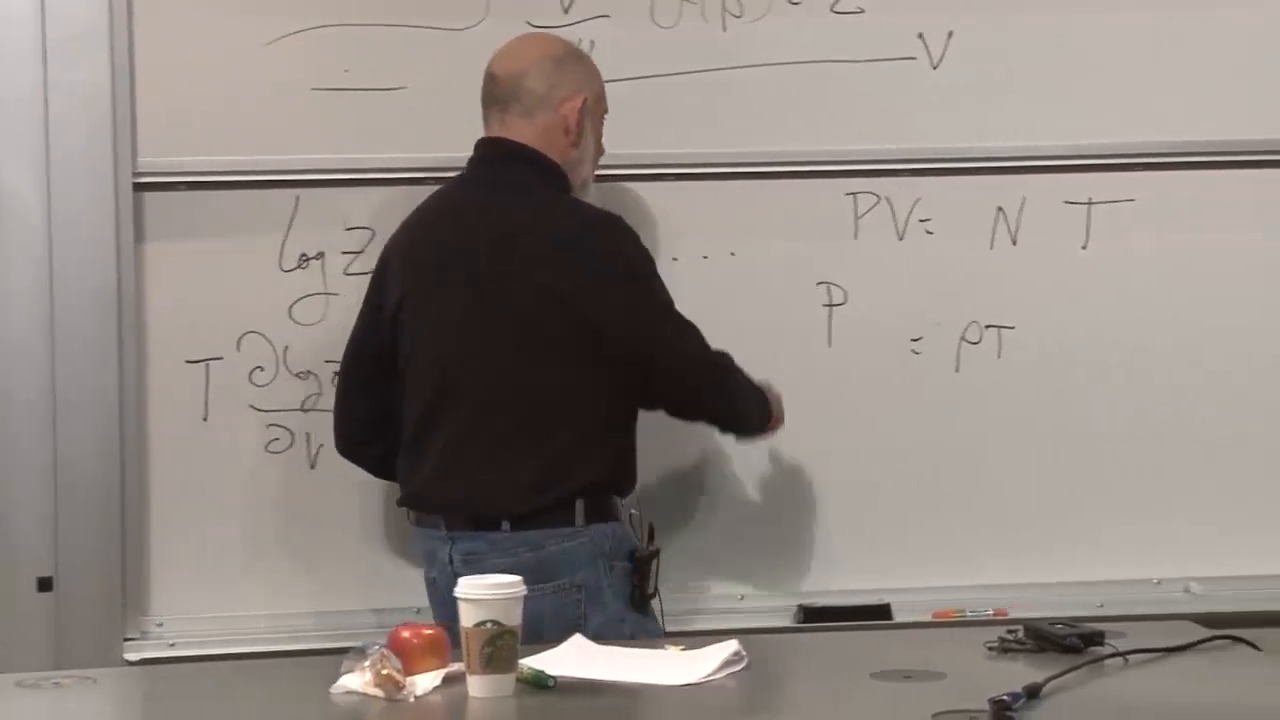
\includegraphics[width=0.90\textwidth]{lecture_05_figure_05.png}\caption{Géométrie du piston et relation de travail obtenue \(dE=-P\,dV\).}\lectureframe{00:43:10}\end{figure}

Deux précisions sont essentielles. Le piston doit se déplacer assez lentement pour que le système reste arbitrairement proche de l’équilibre, et les parois doivent être isolées afin qu’aucune énergie ne soit fournie sous forme de chaleur. Une traction rapide peut être si brusque qu’aucune molécule n’atteigne le piston qui s’éloigne pendant son mouvement. Une compression rapide engendre des ondes de choc. Aucun de ces processus ne peut être décrit comme une succession d’états d’équilibre.

Le terme \emph{adiabatique} désigne parfois l’absence de transfert thermique et parfois une variation lente. Dans le processus réversible requis ici, les deux notions interviennent : la variation est quasi statique et le système est isolé thermiquement. Dans ces conditions, elle est aussi isentropique.

\begin{classroomqa}\audiencequestion{Pourquoi une transformation adiabatique conserve-t-elle l’entropie ?}\lecturerresponse{Considérons le système du point de vue de la mécanique quantique. Ses niveaux d’énergie à plusieurs corps dépendent du volume. Lorsque \(V\) varie lentement, le théorème adiabatique fait évoluer continûment chaque niveau occupé vers le niveau correspondant, sans transition entre les étiquettes des niveaux. Les énergies \(E_i(V)\) varient, mais les probabilités d’occupation \(p_i\) restent fixes. Comme \(S=-\sum_i p_i\log p_i\) dépend de ces probabilités, l’entropie reste constante. Un échange de chaleur ou un mouvement irréversible invaliderait cette conclusion.\lecturetimestamp{00:43:37--00:49:15}}\end{classroomqa}

\begin{figure}[t]\centering
\includegraphics[width=0.90\textwidth]{lecture_05_figure_06.png}\caption{Les niveaux d’énergie à plusieurs corps varient avec le volume tandis que leurs probabilités d’occupation conservent leurs étiquettes de niveau.}\lectureframe{00:48:50}\end{figure}

L’équation \eqref{eq:sm5-adiabatic-work}, évaluée le long de ce chemin à entropie constante, identifie la pression à \begin{equation}
 P=-\left(\frac{\partial E}{\partial V}\right)_S.
 \label{eq:sm5-pressure-fixed-entropy}
\end{equation} C’est la relation de conjugaison entre la pression et le volume.

\begin{classroomqa}\audiencequestion{Que se passe-t-il si le piston se déplace rapidement ?}\lecturerresponse{Le système quitte l’équilibre et sa dynamique détaillée devient pertinente. Une compression brutale engendre une onde de choc. Lors d’une détente libre idéale, le piston peut s’éloigner avant que la moindre molécule ne le heurte : aucun travail n’est alors effectué et l’énergie reste fixe, bien que le volume varie. Le gaz revient ensuite à l’équilibre avec une entropie accrue. Ces processus ne peuvent pas être décrits par l’unique dérivée d’équilibre de \eqref{eq:sm5-pressure-fixed-entropy}.\lecturetimestamp{00:58:30--01:01:15}}\end{classroomqa}

\begin{classroomqa}\audiencequestion{Quelle condition quantitative permet de décider si une variation est lente ?}\lecturerresponse{Le temps caractéristique de la variation extérieure doit être long devant les temps de relaxation internes pertinents. Pour un gaz, de nombreuses collisions moléculaires et de nombreux chocs contre les parois doivent avoir lieu pendant la variation macroscopique. L’échelle de temps précise dépend du matériau et de la géométrie, tandis que la limite quasi statique est générale.\lecturetimestamp{01:02:09--01:03:20}}\end{classroomqa}

\section{De l’énergie adiabatique à la fonction de partition}

La formule physique \eqref{eq:sm5-pressure-fixed-entropy} n’est pas encore la plus facile à calculer. La mécanique statistique canonique fournit naturellement des fonctions de la température, puisque \(T\) apparaît directement dans le facteur de Boltzmann. Le lemme de calcul transforme la dérivée peu commode à entropie fixe en une expression adaptée au calcul : \begin{align}
 P
 &=
 -\left(\frac{\partial E}{\partial V}\right)_T
 +
 \left(\frac{\partial E}{\partial S}\right)_V
 \left(\frac{\partial S}{\partial V}\right)_T.
 \label{eq:sm5-pressure-lemma-substitution}
\end{align} À volume fixe, le premier principe donne \(dE=T\,dS\), et donc \begin{equation}
 \left(\frac{\partial E}{\partial S}\right)_V=T.
 \label{eq:sm5-e-s-temperature}
\end{equation} Ainsi, \begin{equation}
 P=
 -\left(\frac{\partial E}{\partial V}\right)_T
 +
 T\left(\frac{\partial S}{\partial V}\right)_T.
 \label{eq:sm5-pressure-fixed-temperature-pieces}
\end{equation}

\begin{classroomqa}\audiencequestion{D’où vient le signe moins dans la formule de la pression ?}\lecturerresponse{Il provient du travail fourni par le gaz : \(dE=-P\,dV\) lors d’une détente adiabatique. Le lemme de calcul lui-même comporte un signe moins entre ses deux termes ; le signe moins global dans \(P=-(\partial E/\partial V)_S\) inverse les deux, ce qui donne \eqref{eq:sm5-pressure-fixed-temperature-pieces}.\lecturetimestamp{00:52:40--00:53:14}}\end{classroomqa}

Comme \(T\) reste fixe dans les deux dérivées, \begin{align}
 P
 &=
 -\left(\frac{\partial}{\partial V}(E-TS)\right)_T \notag\\
 &=
 -\left(\frac{\partial A}{\partial V}\right)_T.
 \label{eq:sm5-pressure-free-energy}
\end{align} Enfin, introduisons \(A=-T\log Z\) : \begin{equation}
 \boxed{
 P=
 T\left(\frac{\partial\log Z}{\partial V}\right)_T
 }.
 \label{eq:sm5-pressure-log-z}
\end{equation}

\begin{figure}[t]\centering
\includegraphics[width=0.90\textwidth]{lecture_05_figure_07.png}\caption{Le raisonnement à température fixe : \(P=-(\partial A/\partial V)_T
=T(\partial\log Z/\partial V)_T\).}\lectureframe{00:55:55}\end{figure}

Rien dans \eqref{eq:sm5-pressure-log-z} ne suppose que le gaz est parfait. Si l’on peut calculer la fonction de partition d’un fluide avec interactions, d’un plasma ou d’un solide, la même dérivée donne sa pression. Plus généralement, chaque paramètre de contrôle extérieur possède une réponse conjuguée que l’on obtient en dérivant le potentiel thermodynamique approprié. La fonction de partition rassemble bon nombre de ces réponses : sa dérivée \(\log Z\) par rapport à \(\beta\) donne l’énergie, tandis que sa dérivée par rapport au volume donne la pression.

\section{L’équation d’état du gaz parfait}

Spécialisons-nous seulement maintenant au cas de \(N\) particules sans interaction. En conservant la normalisation classique de l’espace des phases, \begin{equation}
 Z_N=
 \frac{1}{N!h^{3N}}
 \int d^{3N}q\,d^{3N}p\,
 \exp\!\left[
 -\beta\sum_{a=1}^{N}\frac{\mathbf p_a^2}{2m}
 \right].
 \label{eq:sm5-ideal-gas-partition-integral}
\end{equation} Il y a \(3N\) coordonnées de position et \(3N\) coordonnées d’impulsion. L’hamiltonien ne dépend pas de la position ; chaque particule apporte donc un facteur égal au volume du récipient : \begin{equation}
 Z_N=
 \frac{V^N}{N!h^{3N}}I_p(\beta),
 \label{eq:sm5-ideal-gas-factorization}
\end{equation} où l’intégrale sur les impulsions entière \(I_p(\beta)\) est indépendante de \(V\).

\begin{classroomqa}\audiencequestion{Pourquoi y a-t-il \(3N\) intégrales sur les positions et \(3N\) intégrales sur les impulsions ?}\lecturerresponse{Chacune des \(N\) particules possède trois coordonnées spatiales et trois composantes d’impulsion conjuguées. Le décompte est de \(3N\) dans chaque moitié de l’espace des phases, et non de \(N\) particules plus \(3N\) autres particules.\lecturetimestamp{01:04:19--01:04:28}}\end{classroomqa}

Un passage au logarithme sépare la dépendance en volume : \begin{equation}
 \log Z_N
 =
 N\log V-\log N!-3N\log h+\log I_p(\beta).
 \label{eq:sm5-log-ideal-gas-partition}
\end{equation} Les facteurs \(1/N!\), \(h^{-3N}\) et \(I_p(\beta)\) sont tous indépendants du volume. Ils importent pour l’entropie absolue et d’autres questions, mais pas pour cette dérivée particulière. Ainsi, \begin{equation}
 \left(\frac{\partial\log Z_N}{\partial V}\right)_T
 =\frac{N}{V}.
 \label{eq:sm5-log-z-volume-derivative}
\end{equation} L’équation \eqref{eq:sm5-pressure-log-z} donne immédiatement \begin{equation}
 P=\frac{NT}{V},
 \qquad
 \boxed{PV=NT}.
 \label{eq:sm5-ideal-gas-law}
\end{equation}

\begin{classroomqa}\audiencequestion{\(N\) compte-t-il encore les répliques utilisées pour déduire la distribution de Boltzmann ?}\lecturerresponse{Non. La construction par répliques était un procédé de dénombrement dans la dérivation précédente ; elle n’intervient plus ici. Dans le présent contexte, \(N\) désigne le nombre de particules physiques dans cet échantillon de gaz.\lecturetimestamp{01:07:38--01:08:05}}\end{classroomqa}

En définissant la densité numérique \begin{equation}
 \rho=\frac{N}{V}
 \label{eq:sm5-number-density}
\end{equation}, on obtient la forme équivalente \begin{equation}
 P=\rho T.
 \label{eq:sm5-density-equation-of-state}
\end{equation}

\begin{classroomqa}\audiencequestion{Faut-il diviser par \(N\) ou par \(V\) pour obtenir l’expression en fonction de la densité ?}\lecturerresponse{Divisez \(PV=NT\) par \(V\) : \(P=(N/V)T=\rho T\). Ici, \(\rho\) désigne la densité numérique, et non la masse volumique.\lecturetimestamp{01:08:45--01:09:16}}\end{classroomqa}

\begin{figure}[t]\centering
\includegraphics[width=0.90\textwidth]{lecture_05_figure_08.png}\caption{La dérivée par rapport au volume de \(\log Z\) et l’équation d’état du gaz parfait qui en résulte, \(PV=NT\), ou \(P=\rho T\).}\lectureframe{01:09:25}\end{figure}

En rétablissant la température de laboratoire \(T_K\), on obtient \begin{equation}
 PV=Nk_BT_K.
 \label{eq:sm5-ideal-gas-law-laboratory}
\end{equation} Le résultat familier concorde avec l’intuition cinétique, mais sa dérivation repose désormais sur un cadre qui s’applique bien au-delà du gaz libre.

\section{Autre résultat : les fluctuations à l’équilibre}

Le calcul de la pression est terminé, mais une question reste en suspens : que peut-on encore tirer de la fonction de partition ? Considérons un système en contact thermique avec un bain. Son énergie n’est pas fixe. L’énergie entre dans le système et en sort ; des mesures répétées fluctuent donc autour de la moyenne canonique.

\begin{classroomqa}\audiencequestion{Pouvons-nous maintenant calculer les fluctuations annoncées ?}\lecturerresponse{Oui. Le temps supplémentaire permet de montrer une nouvelle fois le même principe : les dérivées de \(Z\) encodent des informations thermodynamiques mesurables.\lecturetimestamp{01:10:37--01:10:50}}\end{classroomqa}

\subsection{Variance et écart-type}

Pour une variable aléatoire \(x\) telle que \(\langle x\rangle=0\), une mesure de la largeur de la distribution est \(\langle x^2\rangle\). Pour une distribution quelconque, décalons la variable de sa moyenne : \begin{equation}
 \delta x=x-\langle x\rangle.
 \label{eq:sm5-centered-variable}
\end{equation} Sa moyenne est nulle, \begin{equation}
 \langle\delta x\rangle
 =
 \langle x\rangle-\langle x\rangle=0,
 \label{eq:sm5-centered-mean}
\end{equation} et sa moyenne quadratique vaut \begin{align}
 (\Delta x)^2
 &\equiv
 \left\langle\left(x-\langle x\rangle\right)^2\right\rangle \notag\\
 &=
 \langle x^2\rangle
 -2\langle x\rangle^2
 +\langle x\rangle^2 \notag\\
 &=
 \langle x^2\rangle-\langle x\rangle^2.
 \label{eq:sm5-variance}
\end{align} C’est la variance. Sa racine carrée positive \(\Delta x\) est l’écart-type.

\begin{classroomqa}\audiencequestion{Pourquoi la moyenne de \(x-\langle x\rangle\) est-elle exactement nulle ?}\lecturerresponse{La moyenne est une opération linéaire, et \(\langle x\rangle\) est déjà un nombre. On a donc \(\langle x-\langle x\rangle\rangle
=\langle x\rangle-\langle x\rangle=0\).\lecturetimestamp{01:14:02--01:14:22}}\end{classroomqa}

\begin{classroomqa}\audiencequestion{Quelle différence y a-t-il entre le carré de la fluctuation, la variance, la largeur quadratique moyenne et l’écart-type ?}\lecturerresponse{La variance vaut \((\Delta x)^2=\langle x^2\rangle-\langle x\rangle^2\). L’écart-type est sa racine carrée, \(\Delta x\). Pour une variable de moyenne nulle, l’écart-type est aussi sa valeur quadratique moyenne.\lecturetimestamp{01:16:39--01:18:38}}\end{classroomqa}

\begin{figure}[t]\centering
\includegraphics[width=0.90\textwidth]{lecture_05_figure_09.png}\caption{La variable décentrée et le développement qui donne \((\Delta x)^2=\langle x^2\rangle-\langle x\rangle^2\).}\lectureframe{01:17:20}\end{figure}

\subsection{Moments de l’énergie tirés de la fonction de partition}

Dans l’ensemble canonique, \begin{align}
 \langle E\rangle
 &=
 \frac{1}{Z}\sum_i E_i e^{-\beta E_i} \notag\\
 &=
 -\frac{1}{Z}\frac{\partial Z}{\partial\beta}
 =
 -\frac{\partial\log Z}{\partial\beta}.
 \label{eq:sm5-mean-energy-from-z}
\end{align} Multiplier par un facteur \(E_i\) revient à prendre une dérivée par rapport à \(\beta\), avec un signe moins. Une seconde dérivée produit \(E_i^2\) : \begin{equation}
 \langle E^2\rangle
 =
 \frac{1}{Z}\sum_i E_i^2e^{-\beta E_i}
 =
 \frac{1}{Z}\frac{\partial^2 Z}{\partial\beta^2}.
 \label{eq:sm5-second-energy-moment}
\end{equation} La variance de l’énergie vaut donc \begin{align}
 (\Delta E)^2
 &=
 \langle E^2\rangle-\langle E\rangle^2 \notag\\
 &=
 \frac{1}{Z}\frac{\partial^2Z}{\partial\beta^2}
 -
 \frac{1}{Z^2}
 \left(\frac{\partial Z}{\partial\beta}\right)^2 \notag\\
 &=
 \frac{\partial^2\log Z}{\partial\beta^2}
 =
 -\frac{\partial\langle E\rangle}{\partial\beta}.
 \label{eq:sm5-energy-variance-beta}
\end{align} Une fois encore, une observable d’apparence complexe se ramène à une dérivée de \(\log Z\).

\begin{figure}[t]\centering
\includegraphics[width=0.90\textwidth]{lecture_05_figure_10.png}\caption{La dérivée seconde par rapport à \(\beta\) de \(\log Z\), identifiée à la variance de l’énergie.}\lectureframe{01:29:00}\end{figure}

\subsection{Capacité thermique et amplitude des fluctuations}

Dans les unités du cours \(T=1/\beta\), donc \begin{equation}
 -\frac{\partial}{\partial\beta}
 =
 T^2\frac{\partial}{\partial T}.
 \label{eq:sm5-beta-temperature-derivative}
\end{equation} Définissons, à volume fixe, la capacité thermique de l’échantillon entier par \begin{equation}
 C_V\equiv
 \left(\frac{\partial\langle E\rangle}{\partial T}\right)_V.
 \label{eq:sm5-heat-capacity}
\end{equation} L’équation \eqref{eq:sm5-energy-variance-beta} devient \begin{equation}
 \boxed{(\Delta E)^2=T^2C_V}
 \qquad (k_B=1).
 \label{eq:sm5-energy-fluctuation-lecture-units}
\end{equation} Pour la température de laboratoire \(T_K\), où \(\beta=(k_BT_K)^{-1}\), \begin{equation}
 \boxed{(\Delta E)^2=k_BT_K^2C_V}.
 \label{eq:sm5-energy-fluctuation-laboratory}
\end{equation}

\begin{figure}[t]\centering
\includegraphics[width=0.90\textwidth]{lecture_05_figure_11.png}\caption{Passage de la dérivée par rapport à \(\beta\) à la capacité thermique à volume fixe, avec rétablissement du facteur \(k_B\).}\lectureframe{01:31:10}\end{figure}

\begin{classroomqa}\audiencequestion{Faut-il préciser que la dérivée est prise à volume fixe plutôt qu’à pression fixe ?}\lecturerresponse{Oui. Cette dérivation canonique maintient fixes les paramètres de contrôle extérieurs de l’hamiltonien, y compris \(V\). La grandeur obtenue est \(C_V\). Dans un ensemble à pression constante, le volume et le travail peuvent fluctuer, et il faut utiliser le potentiel thermodynamique correspondant ; on ne peut pas simplement remplacer \(C_V\) par \(C_P\) dans \eqref{eq:sm5-energy-fluctuation-laboratory}.\lecturetimestamp{01:29:01--01:29:28; 01:32:50--01:33:21}}\end{classroomqa}

\begin{classroomqa}\audiencequestion{\(C_V\)est-ce une constante du matériau ?}\lecturerresponse{Pas en général. Elle peut dépendre de la température, du volume, de la phase et de la composition. De plus, \(C_V\) désigne ici la capacité thermique de l’échantillon entier ; c’est une grandeur extensive. On n’obtient une chaleur massique qu’en divisant par la masse, le nombre de particules ou la quantité de matière.\lecturetimestamp{01:31:47--01:32:21; 01:33:23--01:34:55}}\end{classroomqa}

Pour une matière ordinaire extensive, \(C_V\) est proportionnelle à \(N\), donc \((\Delta E)^2\) est proportionnelle à \(N\) et \(\Delta E\) à \(\sqrt{N}\). L’énergie moyenne elle-même est proportionnelle à \(N\). Par conséquent, \begin{equation}
 \frac{\Delta E}{\langle E\rangle}\sim\frac{1}{\sqrt{N}}.
 \label{eq:sm5-relative-fluctuation-scaling}
\end{equation} Les fluctuations relatives sont infimes à l’échelle macroscopique, tandis que les échantillons microscopiques les révèlent directement. La présence de \(k_B\) dans \eqref{eq:sm5-energy-fluctuation-laboratory} marque ce lien entre les observables thermodynamiques et le caractère discret des molécules ; de manière équivalente, elle relie les unités macroscopiques au dénombrement à l’échelle du nombre d’Avogadro.

La pression et les fluctuations découlent désormais d’un même objet : \[
 P=T\left(\frac{\partial\log Z}{\partial V}\right)_T,
 \qquad
 (\Delta E)^2=\frac{\partial^2\log Z}{\partial\beta^2}.
\] C’est la leçon essentielle. Une fois les bonnes contraintes identifiées, la fonction de partition ne sert pas seulement à normaliser les probabilités. Ses dérivées organisent les grandeurs thermodynamiques mesurables du système.